% ============================================================
% Progress Report 2 / Rapport d'Avancement 2 -- PFE Presentation
% An Agentic Framework for IaC Security Analysis and Remediation
%
% Student : Ahmedou Yahye Kheyri
% Supervisor: Prof. Hala Bezine
% Faculte des Sciences de Sfax -- Master MRSI -- 2025-2026
% ============================================================

% Pass xcolor options BEFORE beamer loads xcolor
\PassOptionsToPackage{table,xcdraw,dvipsnames}{xcolor}
\documentclass[aspectratio=169, 10pt]{beamer}

\usetheme{Madrid}
\usecolortheme{default}

% ----------------------------------------------------------------
% Color palette
% ----------------------------------------------------------------
\definecolor{sfaxblue}{RGB}{0,51,102}
\definecolor{sfaxgold}{RGB}{204,153,0}
\definecolor{sfaxlightblue}{RGB}{214,234,248}
\definecolor{sfaxdark}{RGB}{10,30,60}
\definecolor{accentred}{RGB}{180,30,30}
\definecolor{accentgreen}{RGB}{30,130,70}
\definecolor{accentorange}{RGB}{210,100,10}
\definecolor{moduleblue}{RGB}{52,109,163}
\definecolor{moduleorange}{RGB}{200,110,30}
\definecolor{modulepurple}{RGB}{120,60,160}
\definecolor{modulegreen}{RGB}{45,140,80}
\definecolor{modulered}{RGB}{180,50,50}
\definecolor{codebg}{RGB}{245,248,252}
\definecolor{titlebg}{RGB}{0,40,85}

% ----------------------------------------------------------------
% Apply colors to Beamer
% ----------------------------------------------------------------
\setbeamercolor{palette primary}{bg=sfaxblue,fg=white}
\setbeamercolor{palette secondary}{bg=sfaxblue!80,fg=white}
\setbeamercolor{palette tertiary}{bg=sfaxblue!60,fg=white}
\setbeamercolor{palette quaternary}{bg=sfaxgold,fg=sfaxblue}
\setbeamercolor{structure}{fg=sfaxblue}
\setbeamercolor{frametitle}{bg=sfaxblue,fg=white}
\setbeamercolor{title}{fg=white}
\setbeamercolor{block title}{bg=sfaxblue,fg=white}
\setbeamercolor{block body}{bg=sfaxlightblue}
\setbeamercolor{block title alerted}{bg=accentred,fg=white}
\setbeamercolor{block body alerted}{bg=accentred!10}
\setbeamercolor{block title example}{bg=accentgreen,fg=white}
\setbeamercolor{block body example}{bg=accentgreen!10}
\setbeamercolor{item}{fg=sfaxblue}
\setbeamercolor{subitem}{fg=sfaxgold}
\setbeamercolor{section in toc}{fg=sfaxblue}

% ----------------------------------------------------------------
% Packages
% ----------------------------------------------------------------
\usepackage[utf8]{inputenc}
\usepackage[T1]{fontenc}
\usepackage{lmodern}
\usepackage{microtype}
\usepackage{graphicx}
\usepackage{booktabs}
\usepackage{tabularx}
\usepackage{multirow}
\usepackage{array}
\usepackage{colortbl}
\usepackage{tikz}
\usetikzlibrary{shapes.geometric,arrows.meta,positioning,fit,
                backgrounds,calc,decorations.pathreplacing,
                shadows.blur,matrix,chains}
\usepackage{listings}
\usepackage{fontawesome5}
\usepackage{amsmath}
\usepackage{pgfplots}
\pgfplotsset{compat=1.18}
% Shield-alt icon shorthand (free FA5 has no \faShieldAlt macro)
\newcommand{\faShieldAlt}{\faPreselectedIcon{shield-alt}}

% ----------------------------------------------------------------
% Listings style
% ----------------------------------------------------------------
\lstdefinestyle{iac}{
  backgroundcolor=\color{codebg},
  basicstyle=\ttfamily\tiny,
  breaklines=true,
  frame=single,
  rulecolor=\color{sfaxblue!30},
  keywordstyle=\color{sfaxblue}\bfseries,
  stringstyle=\color{accentred},
  commentstyle=\color{accentgreen}\itshape,
  numbers=left,
  numberstyle=\tiny\color{gray},
  numbersep=4pt,
  tabsize=2,
  showstringspaces=false,
}
\lstset{style=iac}

% ----------------------------------------------------------------
% Footline
% ----------------------------------------------------------------
\setbeamertemplate{navigation symbols}{}
\setbeamertemplate{footline}{
  \leavevmode%
  \hbox{%
    \begin{beamercolorbox}[wd=.30\paperwidth,ht=2.5ex,dp=1.5ex,center]{palette secondary}%
      \usebeamerfont{author in head/foot}\textbf{A.Y. Kheyri} --- FSS Sfax
    \end{beamercolorbox}%
    \begin{beamercolorbox}[wd=.40\paperwidth,ht=2.5ex,dp=1.5ex,center]{palette tertiary}%
      \usebeamerfont{title in head/foot}\textit{Agentic IaC Security Framework}
    \end{beamercolorbox}%
    \begin{beamercolorbox}[wd=.30\paperwidth,ht=2.5ex,dp=1.5ex,right]{palette quaternary}%
      \usebeamerfont{date in head/foot}
      Master MRSI --- PFE 2025--2026 \quad
      \insertframenumber{}/\inserttotalframenumber\hspace*{2ex}
    \end{beamercolorbox}}%
}

% ----------------------------------------------------------------
% Itemize bullets
% ----------------------------------------------------------------
\setbeamertemplate{itemize item}{\color{sfaxgold}\textbullet}
\setbeamertemplate{itemize subitem}{\color{sfaxblue}\faAngleRight}

% ----------------------------------------------------------------
% Helper: colored module card (TikZ)
% ----------------------------------------------------------------
\newcommand{\modulecard}[4]{%
  % #1=color, #2=icon, #3=number+title, #4=subtitle
  \begin{tikzpicture}
    \node[draw=#1, fill=#1!15, rounded corners=5pt,
          minimum width=3.6cm, minimum height=1.1cm,
          align=center, text width=3.4cm,
          drop shadow={shadow blur steps=5, opacity=0.2}] (box) at (0,0)
      {{\color{#1}\large#2}\\[2pt]
       {\color{#1}\bfseries\scriptsize#3}\\[1pt]
       {\color{black!70}\tiny#4}};
  \end{tikzpicture}%
}


% ----------------------------------------------------------------
% Title info
% ----------------------------------------------------------------
\title[Agentic IaC Security Framework]{%
  \textbf{An Agentic Framework for IaC\\
  Misconfiguration Analysis and Remediation}}
\subtitle{Progress Report 2 --- PFE Master MRSI}
\author[Ahmedou Yahye Kheyri]{%
  \textbf{Ahmedou Yahye Kheyri}\\[3pt]
  {\small \faUserGraduate\ Supervised by: \textbf{Prof.\ Hala Bezine}}}
\institute[FSS -- Sfax]{%
  \faUniversity\ \textbf{Faculty of Sciences of Sfax}\\
  University of Sfax --- Tunisia\\
  Master MRSI (Reseaux et Systemes Informatiques)}
\date{\faCalendar\ April 2026}

% ================================================================
\begin{document}
% ================================================================

% ----------------------------------------------------------------
% TITLE SLIDE
% ----------------------------------------------------------------
{
\setbeamertemplate{footline}{}
\begin{frame}[plain]

\begin{tikzpicture}[remember picture, overlay]
  % Deep blue background
  \fill[titlebg] (current page.south west) rectangle (current page.north east);
  % Gold accent bar at top
  \fill[sfaxgold] ([yshift=-0.13\paperheight]current page.north west)
    rectangle ([yshift=-0.16\paperheight]current page.north east);
  % Decorative circles (right side)
  \fill[sfaxblue!60, opacity=0.4] ([xshift=0.75\paperwidth, yshift=-0.5\paperheight]
    current page.west) circle (3.2cm);
  \fill[sfaxblue!40, opacity=0.3] ([xshift=0.82\paperwidth, yshift=-0.3\paperheight]
    current page.west) circle (2cm);
  \fill[sfaxgold!70, opacity=0.2] ([xshift=0.88\paperwidth, yshift=-0.7\paperheight]
    current page.west) circle (1.4cm);
  % Bottom accent bar
  \fill[sfaxgold] ([yshift=0.07\paperheight]current page.south west)
    rectangle ([yshift=0.10\paperheight]current page.south east);
\end{tikzpicture}

\begin{columns}[T]
  \begin{column}{0.62\textwidth}
    \vspace{1.2em}
    % University
    
\begin{tikzpicture}
      \node[fill=sfaxgold!20, draw=sfaxgold, rounded corners=3pt,
            minimum width=7cm, minimum height=0.5cm, align=center, font=\tiny\bfseries,
            text=sfaxgold] at (0,0)
        {\faUniversity\ FACULTY OF SCIENCES OF SFAX --- UNIVERSITY OF SFAX};
    \end{tikzpicture}
    \vspace{0.5em}\\
    % Title
    {\color{sfaxgold}\rule{7cm}{1.5pt}}\\[0.5em]
    {\color{white}\large\textbf{An Agentic Framework for IaC}}\\[0.2em]
    {\color{white}\large\textbf{Misconfiguration Analysis}}\\[0.2em]
    {\color{white}\large\textbf{and Automated Remediation}}\\[0.3em]
    {\color{sfaxgold}\rule{7cm}{1.5pt}}\\[1em]
    % Author info box
    \begin{tikzpicture}
      \node[fill=sfaxblue!40, draw=sfaxgold!60, rounded corners=4pt,
            minimum width=7cm, align=left, inner sep=8pt, font=\small] at (0,0) {
        \begin{tabular}{@{}ll@{}}
          {\color{sfaxgold}\faUserGraduate} & {\color{white}\textbf{Ahmedou Yahye Kheyri}}\\[3pt]
          {\color{sfaxgold}\faChalkboardTeacher} & {\color{white!85}Supervised by: \textbf{Prof.\ Hala Bezine}}\\[3pt]
          {\color{sfaxgold}\faGraduationCap} & {\color{white!85}Master MRSI --- PFE 2025--2026}\\[3pt]
          {\color{sfaxgold}\faCalendar} & {\color{white!85}Progress Report 2 --- April 2026}\\
        \end{tabular}
      };
    \end{tikzpicture}
  \end{column}
  \begin{column}{0.35\textwidth}
    \vspace{2em}
    \begin{center}
      % Visual icon cluster
      \begin{tikzpicture}[font=\scriptsize]
        % Central gear
        \node[circle, fill=sfaxgold!80, minimum size=1.2cm, align=center,
              text=sfaxblue] (center) at (0,0)
          {{\large\faCogs}};
        % Surrounding icons
        \node[circle, fill=sfaxblue!60, minimum size=0.8cm, align=center,
              text=white] at (0, 1.7) {{\normalsize\faShieldAlt}};
        \node[circle, fill=accentgreen!60, minimum size=0.8cm, align=center,
              text=white] at (1.5, 0.8) {{\normalsize\faCheckCircle}};
        \node[circle, fill=modulepurple!60, minimum size=0.8cm, align=center,
              text=white] at (1.5,-0.8) {{\normalsize\faDatabase}};
        \node[circle, fill=moduleorange!60, minimum size=0.8cm, align=center,
              text=white] at (0,-1.7) {{\normalsize\faBrain}};
        \node[circle, fill=modulered!60, minimum size=0.8cm, align=center,
              text=white] at (-1.5,-0.8) {{\normalsize\faCode}};
        \node[circle, fill=moduleblue!60, minimum size=0.8cm, align=center,
              text=white] at (-1.5, 0.8) {{\normalsize\faWrench}};
        % Lines
        \foreach \a in {90,30,-30,-90,-150,150}
          \draw[sfaxgold!40, thick] (center) -- +(\a:0.9cm);
      \end{tikzpicture}\\[0.6em]
      {\color{white!70}\tiny\textit{IaC Security $\cdot$ RAG $\cdot$ LLMs $\cdot$ Checkov}}
    \end{center}
  \end{column}
\end{columns}
\end{frame}
}

% ----------------------------------------------------------------
% TABLE OF CONTENTS
% ----------------------------------------------------------------
\begin{frame}{Outline}
  \begin{columns}[T]
    \begin{column}{0.55\textwidth}
      \tableofcontents
    \end{column}
    \begin{column}{0.42\textwidth}
      \begin{center}
        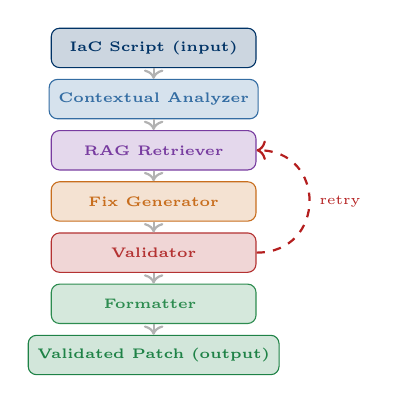
\begin{tikzpicture}[font=\scriptsize,
          every node/.style={align=center}]
          % Pipeline mini-diagram
          \def\bw{2.6cm}
          \def\bh{0.5cm}
          \foreach \i/\col/\lbl in {
            5/moduleblue/Contextual Analyzer,
            4/modulepurple/RAG Retriever,
            3/moduleorange/Fix Generator,
            2/modulered/Validator,
            1/modulegreen/Formatter
          }{
            \node[draw=\col, fill=\col!20, rounded corners=3pt,
                  minimum width=\bw, minimum height=\bh,
                  font=\tiny\bfseries, text=\col] (n\i) at (0, \i*0.65)
              {\lbl};
          }
          \node[draw=sfaxblue, fill=sfaxblue!20, rounded corners=3pt,
                minimum width=\bw, minimum height=\bh,
                font=\tiny\bfseries, text=sfaxblue] (n6) at (0, 6*0.65)
            {IaC Script (input)};
          \node[draw=accentgreen, fill=accentgreen!20, rounded corners=3pt,
                minimum width=\bw, minimum height=\bh,
                font=\tiny\bfseries, text=accentgreen] (n0) at (0, 0)
            {Validated Patch (output)};
          \foreach \a/\b in {6/5,5/4,4/3,3/2,2/1,1/0}
            \draw[->,thick,gray!60] (n\a.south) -- (n\b.north);
          \draw[->,dashed,accentred,thick]
            (n2.east) .. controls (2.2,2*0.65) and (2.2,4*0.65) ..
            node[right,font=\tiny,color=accentred]{retry} (n4.east);
        \end{tikzpicture}
      \end{center}
    \end{column}
  \end{columns}
\end{frame}

% ================================================================
\section{Context \& Motivation}
% ================================================================

% Section transition
{
\setbeamertemplate{footline}{}
\begin{frame}[plain]
\begin{tikzpicture}[remember picture, overlay]
  \fill[sfaxblue] (current page.south west) rectangle (current page.north east);
  \fill[sfaxgold] ([yshift=-0.45\paperheight]current page.north west)
    rectangle ([yshift=-0.55\paperheight]current page.north east);
  \node[text=white, font=\Huge\bfseries] at (current page.center)
    {1. Context \& Motivation};
  \node[text=sfaxgold!80, font=\large] at ([yshift=-1.2cm]current page.center)
    {Why does IaC security matter?};
\end{tikzpicture}
\end{frame}
}

\begin{frame}[shrink=12]{Infrastructure as Code (IaC): The New Attack Surface}
  \begin{columns}[T]
    \begin{column}{0.50\textwidth}
      \begin{block}{\faCode\ What is IaC?}
        Code that \textbf{defines and provisions} cloud infrastructure ---
        servers, networks, databases, firewalls.\\[0.1em]
        \textbf{4 dominant formats:}
        \begin{itemize}
          \item \faCloud\ \textbf{Terraform} (.tf) --- AWS, Azure, GCP
          \item \faServer\ \textbf{Ansible} (.yml) --- configuration mgmt
          \item \faDocker\ \textbf{Kubernetes} (.yaml) --- container orchestration
          \item \faDocker\ \textbf{Dockerfile} --- container images
        \end{itemize}
      \end{block}
      \vspace{0.2em}
      \begin{alertblock}{\faExclamationTriangle\ The Problem}
        IaC scripts are shipped with \textbf{security misconfigurations}.\\
        \textbf{62 categories} of security smells (War et al., 2025):
        hard-coded secrets, open firewall rules, privileged containers...
      \end{alertblock}
    \end{column}
    \begin{column}{0.47\textwidth}
      \begin{center}
      \begin{tikzpicture}[font=\scriptsize]
        % IaC tools on the left
        \foreach \i/\col/\ico/\lbl in {
          3/moduleblue/\faCloud/Terraform (.tf),
          2/modulepurple/\faServer/Ansible (.yml),
          1/sfaxblue/\faDocker/Kubernetes (.yaml),
          0/moduleorange/\faDocker/Dockerfile
        }{
          \node[draw=\col, fill=\col!15, rounded corners=3pt,
                minimum width=2.8cm, minimum height=0.55cm,
                align=center, font=\tiny\bfseries] (tool\i) at (0, \i*0.75)
            {{\color{\col}\ico}\ \lbl};
        }
        % Security smells cloud on the right
        \node[draw=accentred, fill=accentred!10, rounded corners=8pt,
              minimum width=2.6cm, minimum height=2.6cm,
              align=center, text width=2.4cm] (cloud) at (4.0, 1.12)
          {{\color{accentred}\large\faBug}\\[2pt]
           {\color{accentred}\textbf{Security}}\\
           {\color{accentred}\textbf{Smells}}\\[2pt]
           {\tiny\color{black!70}62 categories}\\
           {\tiny\color{black!70}CWE-aligned}};
        % Arrows
        \foreach \i in {0,1,2,3}
          \draw[->,accentred!60,thick] (tool\i.east) -- (cloud.west);
        % Detect-only badge
        \node[draw=gray, fill=gray!15, rounded corners=3pt,
              font=\tiny, align=center, below=0.2cm of cloud] (badge)
          {\faSearch\ Tools \textbf{detect} only\\
           \faTimesCircle\ No automated \textbf{fix}};
      \end{tikzpicture}
      \end{center}
    \end{column}
  \end{columns}
\end{frame}

\begin{frame}{Research Gap \& Our Contribution}
  \begin{columns}[T]
    \begin{column}{0.48\textwidth}
      \begin{alertblock}{\faTimesCircle\ Limitations of Existing Approaches}
        \begin{itemize}
          \item \textbf{Checkov / Terrascan}: detect only, zero fix generation
          \item \textbf{Passive RAG systems}: patches with no validation
          \item \textbf{LLM hallucinations}: wrong patches, no safety net
          \item \textbf{No iterative loop}: one shot, fail silently
        \end{itemize}
      \end{alertblock}
      \vspace{0.5em}
      \begin{center}
        \begin{tikzpicture}[font=\scriptsize]
          \node[draw=sfaxblue, fill=sfaxlightblue, rounded corners=4pt,
                minimum width=5.5cm, minimum height=0.8cm,
                align=center, inner sep=6pt] {
            {\color{sfaxblue}\faQuoteLeft}\
            \textit{Can we close the loop: detect $\to$}\\
            \textit{retrieve $\to$ generate $\to$ validate?}
            \ {\color{sfaxblue}\faQuoteRight}
          };
        \end{tikzpicture}
      \end{center}
    \end{column}
    \begin{column}{0.48\textwidth}
      \begin{exampleblock}{\faLightbulb\ Our Proposed Approach}
        \begin{itemize}
          \item LLM generation + \textbf{external validation}
          \item \textbf{CRAG} (Corrective RAG) --- refines on failure
          \item \textbf{Retry loop} (max 3 attempts)
          \item Validator = Checkov (independent judge)
          \item Target output: validated diff + CWE explanation
        \end{itemize}
      \end{exampleblock}
      \vspace{0.4em}
      % Comparison bar (hardcoded to avoid xcolor foreach issue)
      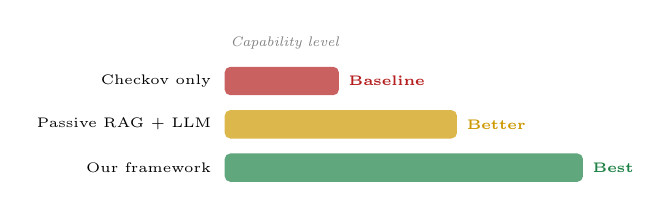
\begin{tikzpicture}[font=\tiny]
        \node[left] at (0, 1.10) {Checkov only};
        \fill[accentred, fill opacity=0.7, rounded corners=2pt]
          (0.05,0.92) rectangle (1.5,1.28);
        \node[right, font=\tiny\bfseries, color=accentred] at (1.5,1.10) {Baseline};
        \node[left] at (0, 0.55) {Passive RAG + LLM};
        \fill[sfaxgold, fill opacity=0.7, rounded corners=2pt]
          (0.05,0.37) rectangle (3.0,0.73);
        \node[right, font=\tiny\bfseries, color=sfaxgold] at (3.0,0.55) {Better};
        \node[left] at (0, 0.00) {Our framework};
        \fill[accentgreen, fill opacity=0.7, rounded corners=2pt]
          (0.05,-0.18) rectangle (4.6,0.18);
        \node[right, font=\tiny\bfseries, color=accentgreen] at (4.6,0.00) {Best};
        \node[above right, font=\tiny\itshape, color=gray] at (0,1.38)
          {Capability level};
      \end{tikzpicture}
    \end{column}
  \end{columns}
\end{frame}

% ================================================================
\section{State of the Art}
% ================================================================

{
\setbeamertemplate{footline}{}
\begin{frame}[plain]
\begin{tikzpicture}[remember picture, overlay]
  \fill[sfaxdark] (current page.south west) rectangle (current page.north east);
  \fill[sfaxgold] ([yshift=-0.45\paperheight]current page.north west)
    rectangle ([yshift=-0.55\paperheight]current page.north east);
  \node[text=white, font=\Huge\bfseries] at (current page.center)
    {2. State of the Art};
  \node[text=sfaxgold!80, font=\large] at ([yshift=-1.2cm]current page.center)
    {From detection to remediation};
\end{tikzpicture}
\end{frame}
}

\begin{frame}{Related Work at a Glance}
  \begin{center}
  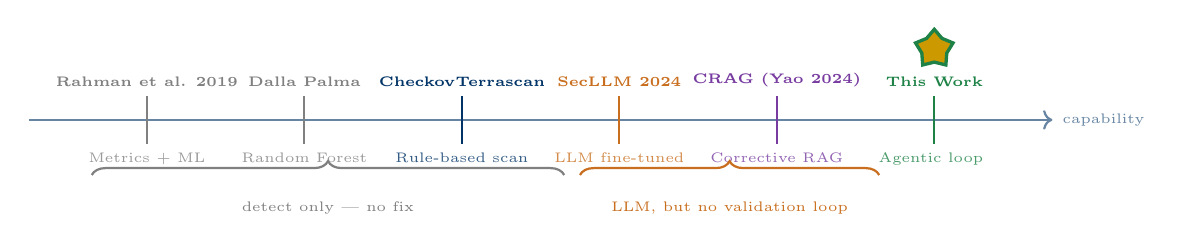
\begin{tikzpicture}[font=\scriptsize]
    % Timeline horizontal
    \draw[->, thick, sfaxblue!60] (-0.5, 0) -- (12.5, 0)
      node[right, font=\tiny] {capability};
    % Levels
    \foreach \x/\col/\lbl/\sub in {
      1.0/gray/Rahman et al. 2019/Metrics + ML,
      3.0/gray/Dalla Palma/Random Forest,
      5.0/sfaxblue/Checkov\/Terrascan/Rule-based scan,
      7.0/moduleorange/SecLLM 2024/LLM fine-tuned,
      9.0/modulepurple/CRAG (Yao 2024)/Corrective RAG,
      11.0/accentgreen/This Work/Agentic loop
    }{
      \draw[\col, thick] (\x,-0.3) -- (\x,0.3);
      \node[above, font=\tiny\bfseries, text=\col, align=center] at (\x,0.3)
        {\lbl};
      \node[below, font=\tiny, text=\col!80, align=center] at (\x,-0.3)
        {\sub};
    }
    % Bracket for "detect only"
    \draw[decorate, decoration={brace,amplitude=5pt}, thick, gray]
      (0.3,-0.7) -- (6.3,-0.7) node[midway,below=6pt,font=\tiny,gray]
      {detect only --- no fix};
    % Bracket for "LLM era"
    \draw[decorate, decoration={brace,amplitude=5pt}, thick, moduleorange]
      (6.5,-0.7) -- (10.3,-0.7) node[midway,below=6pt,font=\tiny,moduleorange]
      {LLM, but no validation loop};
    % Star for this work
    \node[star, star points=5, fill=sfaxgold, minimum size=0.5cm,
          draw=accentgreen, very thick] at (11,0.9) {};
  \end{tikzpicture}
  \end{center}
  \vspace{0.2em}
  \begin{center}
  {\scriptsize
  \begin{tabular}{@{}lllll@{}}
    \toprule
    \textbf{Work} & \textbf{Approach} & \textbf{Coverage}
      & \textbf{Fix?} & \textbf{Validation?}\\
    \midrule
    War et al.\ 2025 & 62-cat taxonomy & Multi-tool & \textcolor{accentred}{\faTimes} & \textcolor{accentred}{\faTimes}\\
    SecLLM 2024 & LLM fine-tuned & Terraform & \textcolor{accentgreen}{\faCheck} & \textcolor{accentred}{\faTimes}\\
    GenSIAC 2024 & Fine-tuned GPT & IaC patches & \textcolor{accentgreen}{\faCheck} & \textcolor{accentred}{\faTimes}\\
    CRAG (Yao) & Corrective RAG & General NLP & \textcolor{accentred}{\faTimes} & \textcolor{accentred}{\faTimes}\\
    \rowcolor{sfaxgold!25}
    \textbf{This work} & \textbf{Agentic RAG+LLM} & \textbf{4 tools}
      & \textcolor{accentgreen}{\textbf{\faCheck}} & \textcolor{accentgreen}{\textbf{\faCheck}}\\
    \bottomrule
  \end{tabular}}
  \end{center}
\end{frame}

% ================================================================
\section{Framework Architecture}
% ================================================================

{
\setbeamertemplate{footline}{}
\begin{frame}[plain]
\begin{tikzpicture}[remember picture, overlay]
  \fill[sfaxblue] (current page.south west) rectangle (current page.north east);
  \fill[sfaxgold] ([yshift=-0.45\paperheight]current page.north west)
    rectangle ([yshift=-0.55\paperheight]current page.north east);
  \node[text=white, font=\Huge\bfseries] at (current page.center)
    {3. Framework Architecture};
  \node[text=sfaxgold!80, font=\large] at ([yshift=-1.2cm]current page.center)
    {6 modules --- 1 agentic loop};
\end{tikzpicture}
\end{frame}
}

\begin{frame}{System Architecture --- The Big Picture}
  \begin{center}
  \begin{tikzpicture}[
    font=\scriptsize,
    box/.style={draw, rounded corners=4pt, minimum width=2.5cm,
                minimum height=0.8cm, align=center, text width=2.3cm,
                drop shadow={shadow blur steps=4, opacity=0.15}},
    arrow/.style={->, thick, >=Stealth},
    retry/.style={->, dashed, very thick, >=Stealth, color=accentred},
  ]
    % Input
    \node[draw=sfaxblue, fill=sfaxblue, rounded corners=4pt,
          minimum width=2.6cm, minimum height=0.7cm,
          align=center, text=white, font=\scriptsize\bfseries] (input) at (0,5)
      {\faFileCode\ IaC Script};

    % Central agent box (background)
    \begin{scope}[on background layer]
      \node[draw=sfaxblue!50, dashed, fill=sfaxblue!5, rounded corners=8pt,
            fit={($(0-1.5,0.4)$)($(9.5,4.4)$)},
            label={[sfaxblue!70, font=\tiny\bfseries, above]north:
              \faRobot\ Central Agent (Orchestrator)}] {};
    \end{scope}

    % Module boxes
    \node[box, fill=moduleblue!20, draw=moduleblue] (ca) at (0,3.5)
      {{\color{moduleblue}\faSearch}\newline\textbf{1. Contextual}\newline Analyzer};
    \node[box, fill=modulepurple!20, draw=modulepurple] (kb) at (3.2,3.5)
      {{\color{modulepurple}\faDatabase}\newline\textbf{2. Knowledge}\newline Base + Retriever};
    \node[box, fill=moduleorange!20, draw=moduleorange] (fg) at (6.4,3.5)
      {{\color{moduleorange}\faBrain}\newline\textbf{3. Fix}\newline Generator};
    \node[box, fill=modulered!20, draw=modulered] (ev) at (6.4,1.8)
      {{\color{modulered}\faShieldAlt}\newline\textbf{4. External}\newline Validator};
    \node[box, fill=modulegreen!20, draw=modulegreen] (pf) at (3.2,1.8)
      {{\color{modulegreen}\faFileCode}\newline\textbf{5. Patch}\newline Formatter};

    % Output
    \node[draw=accentgreen, fill=accentgreen, rounded corners=4pt,
          minimum width=2.6cm, minimum height=0.7cm,
          align=center, text=white, font=\scriptsize\bfseries, text width=2.4cm] (out) at (0,1.8)
      {\faCheck\ Patch + CWE\newline Explanation};

    % Arrows
    \draw[arrow, sfaxblue] (input) -- (ca);
    \draw[arrow, sfaxblue] (ca) -- node[above,font=\tiny,color=sfaxblue]{smells} (kb);
    \draw[arrow, sfaxblue] (kb) -- node[above,font=\tiny,color=sfaxblue]{RAG ctx} (fg);
    \draw[arrow, sfaxblue] (fg) -- node[right,font=\tiny,color=sfaxblue]{patch} (ev);
    \draw[arrow, modulegreen] (ev) -- node[above,font=\tiny,color=accentgreen]{valid} (pf);
    \draw[arrow, accentgreen] (pf) -- (out);

    % Retry
    \draw[retry] (ev.south) .. controls (6.4,0.8) and (3.2,0.8)
      .. node[below,font=\tiny,color=accentred]{refine \& retry (max 3)} (kb.south);

    % Checkov badge
    \node[draw=modulered, fill=white, rounded corners=2pt,
          font=\tiny\bfseries, text=modulered,
          right=0.2cm of ev.east, align=center] {Checkov\newline \faTools};

    % LLM badge
    \node[draw=moduleorange, fill=white, rounded corners=2pt,
          font=\tiny\bfseries, text=moduleorange,
          right=0.2cm of fg.east, align=center] {Claude/\newline GPT/Llama};
  \end{tikzpicture}
  \end{center}
\end{frame}

\begin{frame}[fragile]{Module 1 -- Contextual Analyzer}
  \begin{columns}[T]
    \begin{column}{0.50\textwidth}
      \begin{block}{\faSearch\ Role \& Approach}
        \begin{enumerate}
          \item Detect \textbf{IaC tool type} (extension + regex)
          \item Run \textbf{Checkov} $\to$ parse JSON failures
          \item Extract \textbf{metrics}: lines, tokens, blank/comment count
          \item \textbf{Fallback}: regex heuristics if Checkov unavailable
        \end{enumerate}
      \end{block}
      \vspace{0.4em}
      \begin{tikzpicture}[font=\tiny]
        \foreach \i/\col/\lbl/\cwe in {
          3/moduleblue/hardcoded password/CWE-259,
          2/accentred/open CIDR 0.0.0.0\/0/CWE-732,
          1/moduleorange/privileged container/CWE-250,
          0/modulepurple/TLS disabled/CWE-295
        }{
          \node[draw=\col, fill=\col!10, rounded corners=2pt,
                minimum width=4.5cm, minimum height=0.42cm,
                align=left, inner sep=4pt] at (0, \i*0.52)
            {{\color{\col}\faBug}\ \lbl \hfill {\color{\col!70}\texttt{\cwe}}};
        }
        \node[above, font=\tiny\bfseries, color=sfaxblue] at (0, 3*0.52+0.35)
          {Heuristic smell patterns (fallback)};
      \end{tikzpicture}
    \end{column}
    \begin{column}{0.46\textwidth}
\begin{lstlisting}[language=Python, caption=Tool detection logic]
TOOL_SIGNATURES = {
  "terraform": [
    r'resource\s+"',
    r'provider\s+"',
    r'terraform\s*\{'],
  "kubernetes": [
    r"apiVersion:",
    r"kind:\s+Deployment"],
  "ansible": [
    r"^\s*-\s+name:",
    r"^\s*hosts:"],
  "docker": [
    r"^FROM\s+",
    r"^RUN\s+"],
}
# Then: subprocess.run(["checkov",
#   "--file", str(path),
#   "--output", "json", "--quiet"])
\end{lstlisting}
    \end{column}
  \end{columns}
\end{frame}

\begin{frame}[shrink=8]{Modules 2 \& 3 -- Knowledge Base \& RAG Retriever}
  \begin{columns}[T]
    \begin{column}{0.48\textwidth}
      \begin{block}{\faDatabase\ Knowledge Base (ChromaDB)}
        \begin{itemize}
          \item \textbf{62-category} taxonomy (War et al., 2025)
          \item Embeddings: \texttt{all-MiniLM-L6-v2} (80MB, free)
          \item Each document: name + category + description + CWE + fix example
        \end{itemize}
      \end{block}
      \vspace{0.5em}
      \begin{exampleblock}{\faSync\ CRAG Retrieval Strategy}
        \begin{tabular}{@{}cl@{}}
          \textbf{Try} & \textbf{Query Augmentation}\\
          \midrule
          1 & Direct smell descriptions\\
          2 & + ``minimal targeted changes''\\
          3 & + ``most conservative fix''\\
        \end{tabular}\\[0.3em]
        {\scriptsize Each retry gets more conservative to break the LLM out of its failure mode.}
      \end{exampleblock}
    \end{column}
    \begin{column}{0.48\textwidth}
      \vspace{0.5em}
      \begin{tikzpicture}[font=\scriptsize]
        % Document icons
        \foreach \i/\col in {1/sfaxblue, 2/modulepurple, 3/sfaxblue,
                              4/modulepurple, 5/sfaxblue} {
          \node[draw=\col, fill=\col!10, rounded corners=2pt,
                minimum width=1.2cm, minimum height=0.5cm,
                align=center, font=\tiny] (doc\i)
            at ({(\i-3)*1.35}, 2.8) {Doc \i\newline {\color{\col!70}\tiny CWE-xxx}};
        }
        % Query node
        \node[draw=sfaxgold, fill=sfaxgold!15, rounded corners=3pt,
              minimum width=4.2cm, minimum height=0.55cm,
              align=center, font=\tiny\bfseries] (q) at (0, 1.6)
          {\faSearch\ RAG Query (smell-aware)};
        % ChromaDB
        \node[draw=modulepurple, fill=modulepurple!15, rounded corners=5pt,
              minimum width=4.2cm, minimum height=0.6cm,
              align=center, font=\tiny\bfseries] (db) at (0, 0.85)
          {{\color{modulepurple}\faDatabase}\ ChromaDB (all-MiniLM-L6-v2)};
        % Result
        \node[draw=accentgreen, fill=accentgreen!10, rounded corners=3pt,
              minimum width=4.2cm, minimum height=0.55cm,
              align=center, font=\tiny] (out) at (0,0.1)
          {{\color{accentgreen}\faCheck}\ Top-5 docs $\to$ context string};
        % Arrows
        \foreach \i in {1,2,3,4,5}
          \draw[->,sfaxblue!50] (doc\i.south) -- (db.north);
        \draw[->,sfaxblue,thick] (q) -- (db);
        \draw[->,accentgreen,thick] (db) -- (out);
        % CRAG label placed above query to avoid overflow
        \node[above=0.05cm of q, font=\tiny, color=accentred, align=center]
          {{\color{accentred}\faSync}\ CRAG: retry refines query};
      \end{tikzpicture}
    \end{column}
  \end{columns}
\end{frame}

\begin{frame}[fragile]{Module 4 -- Fix Generator (LLM)}
  \begin{columns}[T]
    \begin{column}{0.50\textwidth}
      \begin{block}{\faBrain\ Multi-Backend LLM Support}
        {\scriptsize
        \begin{tabular}{@{}lll@{}}
          \textbf{Env Var} & \textbf{Backend} & \textbf{Default model}\\
          \midrule
          \texttt{ANTHROPIC\_...} & Anthropic & claude-sonnet-4-6\\
          \texttt{OPENROUTER\_...} & OpenRouter & llama-3.1-8b:free\\
          \texttt{MINIMAX\_...} & MiniMax & MiniMax-Text-01\\
          \texttt{OPENAI\_...} & OpenAI & gpt-4o-mini\\
        \end{tabular}
        }\\[0.3em]
        Auto-detected from env, \textbf{no code change} needed.
      \end{block}
      \vspace{0.4em}
      \begin{alertblock}{\faFilter\ Confidence Filtering (SecLLM)}
        LLM appends: \texttt{CONFIDENCE: 0.0--1.0}\\
        Threshold $\geq 0.6$ to proceed.\\
        Temperature $= 0.2$ for determinism.
      \end{alertblock}
    \end{column}
    \begin{column}{0.46\textwidth}
\begin{lstlisting}[caption=Prompt sent to LLM]
[SYSTEM]
You are an IaC security expert.
Output ONLY unified diff format.
Minimal change. No refactoring.
Then: CONFIDENCE: 0.0-1.0

[USER]
## IaC Tool: terraform
## Detected Smells:
- Line 5: hardcoded_credential
  [CWE-798]
## Relevant Security Knowledge:
[Doc 1] CWE=CWE-798
  Smell: Hardcoded Credentials
  Fix: Use env vars or Vault...
## Original Script:
resource "aws_instance" "app" {
  access_key = "AKIA1234..."
}
\end{lstlisting}
    \end{column}
  \end{columns}
\end{frame}

\begin{frame}[shrink=8]{Module 5 -- External Validator (The Key Innovation)}
  \begin{columns}[T]
    \begin{column}{0.48\textwidth}
      \begin{alertblock}{\faShieldAlt\ Why This Module is Critical}
        This is what makes the framework \textbf{active}, not passive.\\[0.3em]
        The LLM output is \textbf{never trusted} without verification by an independent, certified static analysis tool.
      \end{alertblock}
      \vspace{0.4em}
      \begin{block}{\faCalculator\ Validation Criterion}
        Patch is \textbf{valid} iff:
        \[ \text{smell\_ids} \subseteq \text{removed} \;\wedge\;
           \text{new\_issues} = \emptyset \]
        \begin{itemize}
          \item All targeted Checkov IDs must disappear
          \item No new failures introduced
        \end{itemize}
      \end{block}
    \end{column}
    \begin{column}{0.48\textwidth}
      \begin{center}
      \begin{tikzpicture}[font=\scriptsize, node distance=0.45cm]
        \node[draw=sfaxblue, fill=sfaxblue!15, rounded corners=3pt,
              minimum width=3.4cm, minimum height=0.55cm, align=center] (orig)
          {\faFileCode\ Original IaC File};
        \node[draw=moduleorange, fill=moduleorange!15, rounded corners=3pt,
              minimum width=3.4cm, minimum height=0.55cm, align=center,
              below=0.4cm of orig] (applyp)
          {\faCodeBranch\ Apply Patch $\to$ Temp File};
        % Two-column Checkov
        \node[draw=modulered, fill=modulered!10, rounded corners=3pt,
              minimum width=1.5cm, minimum height=0.55cm, align=center,
              below left=0.4cm and -0.85cm of applyp] (ckv1)
          {Checkov\newline (original)};
        \node[draw=modulered, fill=modulered!10, rounded corners=3pt,
              minimum width=1.5cm, minimum height=0.55cm, align=center,
              below right=0.4cm and -0.85cm of applyp] (ckv2)
          {Checkov\newline (patched)};
        \node[draw=sfaxblue, fill=sfaxblue!10, rounded corners=3pt,
              minimum width=3.4cm, minimum height=0.55cm, align=center,
              below=1.7cm of applyp] (cmp)
          {\faBalanceScale\ Compare IDs: removed? new?};
        % Result paths
        \node[draw=accentgreen, fill=accentgreen!15, rounded corners=3pt,
              minimum width=1.5cm, minimum height=0.5cm, align=center,
              below left=0.4cm and -0.85cm of cmp] (ok)
          {{\color{accentgreen}\faCheckCircle}\ Valid};
        \node[draw=accentred, fill=accentred!10, rounded corners=3pt,
              minimum width=1.5cm, minimum height=0.5cm, align=center,
              below right=0.4cm and -0.85cm of cmp] (fail)
          {{\color{accentred}\faTimesCircle}\ Retry};
        % Arrows
        \draw[->,sfaxblue,thick] (orig)--(applyp);
        \draw[->,modulered,thick] (applyp.south west) -- (ckv1.north);
        \draw[->,modulered,thick] (applyp.south east) -- (ckv2.north);
        \draw[->,sfaxblue,thick] (ckv1.south) -- (cmp.north west);
        \draw[->,sfaxblue,thick] (ckv2.south) -- (cmp.north east);
        \draw[->,accentgreen,thick] (cmp.south west) -- (ok.north);
        \draw[->,accentred,thick] (cmp.south east) -- (fail.north);
      \end{tikzpicture}
      \end{center}
    \end{column}
  \end{columns}
\end{frame}

% ================================================================
\section{Evaluation Dataset}
% ================================================================

{
\setbeamertemplate{footline}{}
\begin{frame}[plain]
\begin{tikzpicture}[remember picture, overlay]
  \fill[sfaxdark] (current page.south west) rectangle (current page.north east);
  \fill[sfaxgold] ([yshift=-0.45\paperheight]current page.north west)
    rectangle ([yshift=-0.55\paperheight]current page.north east);
  \node[text=white, font=\Huge\bfseries] at (current page.center)
    {4. Evaluation Dataset};
  \node[text=sfaxgold!80, font=\large] at ([yshift=-1.2cm]current page.center)
    {8 files $\cdot$ 27 labelled smells $\cdot$ 4 IaC tools};
\end{tikzpicture}
\end{frame}
}

\begin{frame}[shrink=8]{Dataset Composition \& Coverage}
  \begin{columns}[T]
    \begin{column}{0.44\textwidth}
      \begin{block}{\faTable\ Dataset v1.0}
        \begin{tabular}{@{}lccc@{}}
          \toprule
          \textbf{Tool} & \textbf{Files} & \textbf{Smells} & \textbf{\%}\\
          \midrule
          \faCloud\ Terraform & 3 & 11 & 41\%\\
          \faServer\ Ansible & 2 & 7 & 26\%\\
          \faDocker\ Kubernetes & 2 & 8 & 30\%\\
          \faDocker\ Docker & 1 & 5 & 19\%\\
          \midrule
          \textbf{Total} & \textbf{8} & \textbf{27} & 100\%\\
          \bottomrule
        \end{tabular}\\[0.3em]
        Each smell: CWE + Checkov ID + line number
      \end{block}
      \vspace{0.3em}
      \begin{exampleblock}{\faCheckCircle\ Quality Checks}
        \begin{itemize}
          \item All smells in 62-category taxonomy
          \item Manually verified with Checkov
          \item 40+ Checkov detection tests pass
        \end{itemize}
      \end{exampleblock}
    \end{column}
    \begin{column}{0.52\textwidth}
      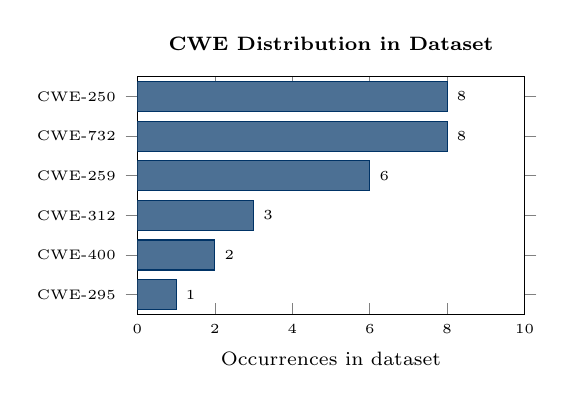
\begin{tikzpicture}
        % CWE bar chart
        \begin{axis}[
          xbar, xmin=0, xmax=10,
          width=6.5cm, height=4.6cm,
          bar width=0.38cm,
          xlabel={\scriptsize Occurrences in dataset},
          symbolic y coords={CWE-295,CWE-400,CWE-312,CWE-259,CWE-732,CWE-250},
          ytick=data,
          nodes near coords,
          nodes near coords align={horizontal},
          every node near coord/.style={font=\tiny},
          tick label style={font=\tiny},
          label style={font=\tiny},
          xlabel style={font=\tiny},
          title={\scriptsize CWE Distribution in Dataset},
          title style={font=\scriptsize\bfseries},
        ]
          \addplot[fill=sfaxblue!70, draw=sfaxblue] coordinates {
            (1,CWE-295) (2,CWE-400) (3,CWE-312)
            (6,CWE-259) (8,CWE-732) (8,CWE-250)
          };
        \end{axis}
      \end{tikzpicture}
      \vspace{0.1em}\\
      {\tiny\color{sfaxblue} CWE-250: Unnecessary Privileges $\cdot$
      CWE-732: Incorrect Permission Assignment $\cdot$
      CWE-259: Hard-coded Password}
    \end{column}
  \end{columns}
\end{frame}

\begin{frame}[fragile]{Dataset: Terraform S3 Example}
  \begin{columns}[T]
    \begin{column}{0.50\textwidth}
\begin{lstlisting}[caption=insecure\_s3.tf --- 4 smells]
resource "aws_s3_bucket" "data" {
  bucket = "my-insecure-bucket"
  acl    = "public-read"  # CWE-732
  # Missing: encryption,
  # versioning, access block
}
resource "aws_s3_bucket_policy" "d" {
  policy = jsonencode({
    Statement = [{
      Principal = "*" # open to all!
      Action    = "s3:*"
    }]
  })
}
\end{lstlisting}
    \end{column}
    \begin{column}{0.47\textwidth}
      \begin{tikzpicture}[font=\tiny]
        \node[draw=accentred, fill=accentred!10, rounded corners=2pt,
              minimum width=5.2cm, minimum height=0.52cm,
              align=left, inner sep=3pt] at (0, 3*0.62)
          {{\color{accentred}\faBug}\ \texttt{overly\_permissive\_acl}\\
           {\color{accentred!70}\texttt{CWE-732} $\cdot$ \texttt{CKV\_AWS\_20}}};
        \node[draw=moduleorange, fill=moduleorange!10, rounded corners=2pt,
              minimum width=5.2cm, minimum height=0.52cm,
              align=left, inner sep=3pt] at (0, 2*0.62)
          {{\color{moduleorange}\faBug}\ \texttt{missing\_encryption}\\
           {\color{moduleorange!70}\texttt{CWE-312} $\cdot$ \texttt{CKV\_AWS\_145}}};
        \node[draw=modulepurple, fill=modulepurple!10, rounded corners=2pt,
              minimum width=5.2cm, minimum height=0.52cm,
              align=left, inner sep=3pt] at (0, 1*0.62)
          {{\color{modulepurple}\faBug}\ \texttt{versioning\_disabled}\\
           {\color{modulepurple!70}\texttt{CWE-284} $\cdot$ \texttt{CKV\_AWS\_21}}};
        \node[draw=sfaxblue, fill=sfaxblue!10, rounded corners=2pt,
              minimum width=5.2cm, minimum height=0.52cm,
              align=left, inner sep=3pt] at (0, 0)
          {{\color{sfaxblue}\faBug}\ \texttt{public\_access\_block}\\
           {\color{sfaxblue!70}\texttt{CWE-732} $\cdot$ \texttt{CKV2\_AWS\_6}}};
        \node[above, font=\tiny\bfseries, color=sfaxblue] at (0, 3*0.62+0.38)
          {Ground-truth smells --- insecure\_s3.tf};
      \end{tikzpicture}
      \vspace{0.15em}
      \begin{exampleblock}{\faVial\ All 58 Tests Pass}
        {\tiny\texttt{pytest tests/ -v} ---
        \textbf{58 passed} in 3m29s}
      \end{exampleblock}
    \end{column}
  \end{columns}
\end{frame}

% ================================================================
\section{Evaluation Methodology}
% ================================================================

{
\setbeamertemplate{footline}{}
\begin{frame}[plain]
\begin{tikzpicture}[remember picture, overlay]
  \fill[sfaxblue] (current page.south west) rectangle (current page.north east);
  \fill[sfaxgold] ([yshift=-0.45\paperheight]current page.north west)
    rectangle ([yshift=-0.55\paperheight]current page.north east);
  \node[text=white, font=\Huge\bfseries] at (current page.center)
    {5. Evaluation Methodology};
  \node[text=sfaxgold!80, font=\large] at ([yshift=-1.2cm]current page.center)
    {4 layers $\cdot$ 18 metrics $\cdot$ ablation study};
\end{tikzpicture}
\end{frame}
}

\begin{frame}[shrink=8]{4-Layer Evaluation Framework}
  \begin{tikzpicture}[font=\scriptsize]
    % Layer boxes
    \foreach \i/\col/\ico/\title/\metrics in {
      3/moduleblue/\faSearchPlus/Layer 1 -- Detection/
        {Precision $\cdot$ Recall $\cdot$ F1 $\cdot$ Macro-F1 per tool \& smell type},
      2/modulepurple/\faProjectDiagram/Layer 2 -- Retrieval/
        {Hit Rate@1 $\cdot$ Hit Rate@3 $\cdot$ Hit Rate@5 $\cdot$ MRR@5 $\cdot$ RAGAS},
      1/moduleorange/\faWrench/Layer 3 -- Remediation/
        {PVR (Patch Validity Rate) $\cdot$ SER $\cdot$ NNIR $\cdot$ Confidence Calibration},
      0/modulegreen/\faRobot/Layer 4 -- Agentic Loop/
        {FA-SR (First-Attempt) $\cdot$ $\Delta$R@2 $\cdot$ $\Delta$R@3 $\cdot$ Fleiss' $\kappa$}
    }{
      \node[draw=\col, fill=\col!12, rounded corners=4pt,
            minimum width=14cm, minimum height=0.78cm,
            text width=13.5cm, align=left, inner sep=5pt] at (7, \i*1.0) {
        {\color{\col}\ico}\quad
        \textcolor{\col}{\textbf{\title}}
        \hfill {\color{black!65}\metrics}
      };
    }
  \end{tikzpicture}
  \vspace{0.3em}
  \begin{columns}[T]
    \begin{column}{0.50\textwidth}
      \begin{block}{\faFlask\ Ablation Study}
        \begin{tabular}{@{}cl@{}}
          \textbf{Config} & \textbf{Description}\\
          \midrule
          A & Checkov only (no LLM) --- \textit{baseline}\\
          B & LLM only, no RAG\\
          C & LLM + passive RAG (no retry)\\
          D & \textbf{Full pipeline (CRAG + Validator)}\\
        \end{tabular}
      \end{block}
    \end{column}
    \begin{column}{0.46\textwidth}
      \begin{block}{\faQuestionCircle\ Research Questions}
        \begin{itemize}
          \item RQ1: Detection accuracy vs ground truth?
          \item RQ2: RAG retrieval quality?
          \item RQ3: Patch validity + smell elimination?
          \item RQ4: Retry loop benefit ($\Delta$R@2, $\Delta$R@3)?
        \end{itemize}
      \end{block}
    \end{column}
  \end{columns}
\end{frame}

% ================================================================
\section{Experimental Results}
% ================================================================

{
\setbeamertemplate{footline}{}
\begin{frame}[plain]
\begin{tikzpicture}[remember picture, overlay]
  \fill[sfaxdark] (current page.south west) rectangle (current page.north east);
  \fill[sfaxgold] ([yshift=-0.45\paperheight]current page.north west)
    rectangle ([yshift=-0.55\paperheight]current page.north east);
  \node[text=white, font=\Huge\bfseries] at (current page.center)
    {6. Experimental Results};
  \node[text=sfaxgold!80, font=\large] at ([yshift=-1.2cm]current page.center)
    {Config A baseline --- Checkov detection analysis};
\end{tikzpicture}
\end{frame}
}

\begin{frame}{Layer 1 -- Detection Results (Config A)}
  \begin{columns}[T]
    \begin{column}{0.46\textwidth}
      \begin{block}{\faTable\ Overall Metrics}
        {\scriptsize
        \begin{tabular}{@{}lcc@{}}
          \toprule
          Metric & Value & Target\\
          \midrule
          True Positives & 7 & ---\\
          False Positives & 76 & ---\\
          False Negatives & 16 & ---\\
          \midrule
          Precision & 0.084 & $>0.85$\\
          Recall & 0.304 & $>0.85$\\
          F1-Score & 0.132 & $>0.80$\\
          Macro-F1 & 0.082 & $>0.80$\\
          \bottomrule
        \end{tabular}}\\[0.3em]
        {\tiny\color{accentred}
        \faBug\ Low precision: Checkov detects 83 checks
        vs only 23 in ground truth.
        This is \textbf{expected} --- Config D will improve this.}
      \end{block}
    \end{column}
    \begin{column}{0.50\textwidth}
      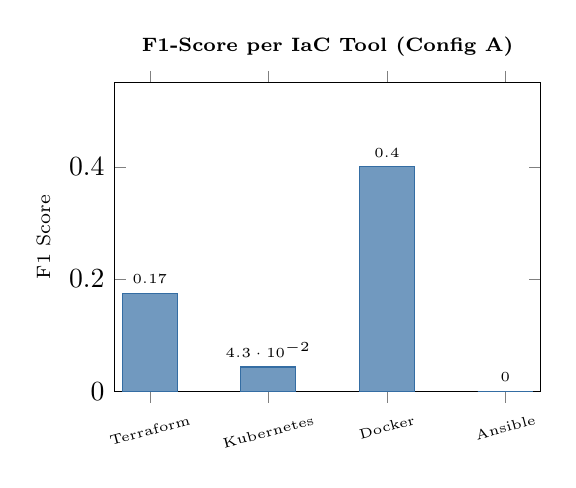
\begin{tikzpicture}
        \begin{axis}[
          ybar, width=7cm, height=5.5cm,
          bar width=0.7cm,
          ylabel={\scriptsize F1 Score},
          xtick={1,2,3,4},
          xticklabels={Terraform,Kubernetes,Docker,Ansible},
          xticklabel style={font=\tiny, rotate=15},
          ymin=0, ymax=0.55,
          ylabel style={font=\tiny},
          title={\scriptsize F1-Score per IaC Tool (Config A)},
          title style={font=\scriptsize\bfseries},
          nodes near coords,
          every node near coord/.style={font=\tiny},
        ]
          \addplot[fill=moduleblue!70, draw=moduleblue] coordinates
            {(1,0.174) (2,0.043) (3,0.400) (4,0.000)};
        \end{axis}
      \end{tikzpicture}
      {\tiny\color{sfaxblue}
      Docker leads (F1=0.40). Ansible=0: smells lack Checkov IDs.
      $\Rightarrow$ GLITCH needed for Ansible.}
    \end{column}
  \end{columns}
\end{frame}

\begin{frame}{Layers 2, 3 \& 4 -- Retrieval and Pending}
  \begin{columns}[T]
    \begin{column}{0.46\textwidth}
      \begin{exampleblock}{\faProjectDiagram\ Layer 2 -- Retrieval}
        {\scriptsize
        \begin{tabular}{@{}lcc@{}}
          \toprule
          Metric & Value & Target\\
          \midrule
          Hit Rate @ K=1 & \textbf{1.000} & $>0.60$\\
          Hit Rate @ K=3 & \textbf{1.000} & $>0.70$\\
          Hit Rate @ K=5 & \textbf{1.000} & $>0.80$\\
          MRR @ K=5 & \textbf{1.000} & $>0.70$\\
          Total queries & 32 & ---\\
          \bottomrule
        \end{tabular}}\\[0.3em]
        {\tiny Keyword-based approximation over the 62-entry taxonomy.
        Full RAGAS metrics require ChromaDB integration.}
      \end{exampleblock}
    \end{column}
    \begin{column}{0.50\textwidth}
      \begin{alertblock}{\faHourglassHalf\ Layers 3 \& 4 --- Pending (LLM)}
        {\scriptsize
        \begin{tabular}{@{}lccc@{}}
          \toprule
          Metric & Config A & Config D target\\
          \midrule
          PVR & 0.000 & $>0.70$\\
          SER & 0.000 & $>0.80$\\
          NNIR & 0.000 & $>0.90$\\
          FA-SR & 0.000 & $>0.50$\\
          $\Delta$R@3 & 0.000 & $>0.10$\\
          \bottomrule
        \end{tabular}}
      \end{alertblock}
      \vspace{0.3em}
      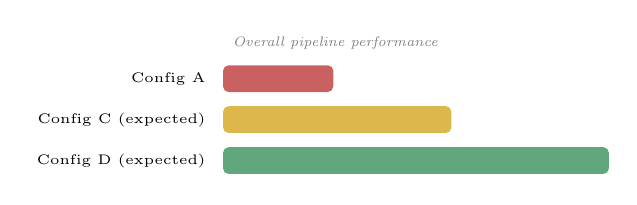
\begin{tikzpicture}[font=\tiny]
        \node[left] at (0,1.04) {Config A};
        \fill[accentred, fill opacity=0.7, rounded corners=2pt]
          (0.1,0.87) rectangle (1.5,1.21);
        \node[left] at (0,0.52) {Config C (expected)};
        \fill[sfaxgold, fill opacity=0.7, rounded corners=2pt]
          (0.1,0.35) rectangle (3.0,0.69);
        \node[left] at (0,0.00) {Config D (expected)};
        \fill[accentgreen, fill opacity=0.7, rounded corners=2pt]
          (0.1,-0.17) rectangle (5.0,0.17);
        \node[above right, font=\tiny\itshape, color=gray] at (0.1, 1.29)
          {Overall pipeline performance};
      \end{tikzpicture}
    \end{column}
  \end{columns}
\end{frame}

% ================================================================
\section{Implementation Status}
% ================================================================

{
\setbeamertemplate{footline}{}
\begin{frame}[plain]
\begin{tikzpicture}[remember picture, overlay]
  \fill[sfaxblue] (current page.south west) rectangle (current page.north east);
  \fill[sfaxgold] ([yshift=-0.45\paperheight]current page.north west)
    rectangle ([yshift=-0.55\paperheight]current page.north east);
  \node[text=white, font=\Huge\bfseries] at (current page.center)
    {7. Implementation Status};
  \node[text=sfaxgold!80, font=\large] at ([yshift=-1.2cm]current page.center)
    {modules under development $\cdot$ baseline results $\cdot$ next steps};
\end{tikzpicture}
\end{frame}
}

\begin{frame}[shrink=5]{Progress Overview}
  % Module status grid
  \begin{center}
  \begin{tikzpicture}[font=\scriptsize]
    \foreach \i/\col/\ico/\title/\status in {
      5/moduleblue/\faSearch/Contextual Analyzer/Done,
      4/modulepurple/\faDatabase/Knowledge Base/Done,
      3/modulepurple/\faProjectDiagram/RAG Retriever/Done,
      2/moduleorange/\faBrain/Fix Generator/In Progress,
      1/modulered/\faShieldAlt/External Validator/Testing,
      0/modulegreen/\faFileCode/Patch Formatter/In Progress
    }{
      \node[draw=\col, fill=\col!15, rounded corners=4pt,
            minimum width=3.8cm, minimum height=0.9cm,
            align=center, text width=3.6cm, inner sep=4pt] (m\i)
        at ({mod(\i,3)*4.2}, {int(\i/3)*1.1}) {
          {\color{\col}\ico}\quad
          {\color{\col}\textbf{\title}}\\
          {\color{accentgreen}\faCheckCircle}\ \textit{\status}
        };
    }
  \end{tikzpicture}
  \end{center}
  \vspace{0.3em}
  \begin{columns}[T]
    \begin{column}{0.48\textwidth}
      \begin{exampleblock}{\faCheckSquare\ Progress So Far}
        \begin{itemize}
          \item \textbf{3/6 modules} fully implemented; 3 under testing
          \item \textbf{58 unit tests} passing (3m29s)
          \item Dataset built: 8 files, 27 labelled smells, 62-cat taxonomy
          \item Evaluation script: baseline mode running
          \item Baseline results (Config A) computed and analysed
        \end{itemize}
      \end{exampleblock}
    \end{column}
    \begin{column}{0.46\textwidth}
      \begin{alertblock}{\faHourglassHalf\ Planned Next Steps}
        \begin{itemize}
          \item Run \textbf{Config D} --- will test LLM fix generation
          \item Populate ChromaDB; plan to measure RAGAS metrics
          \item Explore \textbf{GLITCH} for Ansible/Chef smells
          \item Plan ablation study (B, C, D comparison)
          \item Consider fine-tuning on GenSIAC dataset
        \end{itemize}
      \end{alertblock}
    \end{column}
  \end{columns}
\end{frame}

\begin{frame}[fragile]{Implementation Timeline}
  % 4-phase timeline
  \begin{center}
  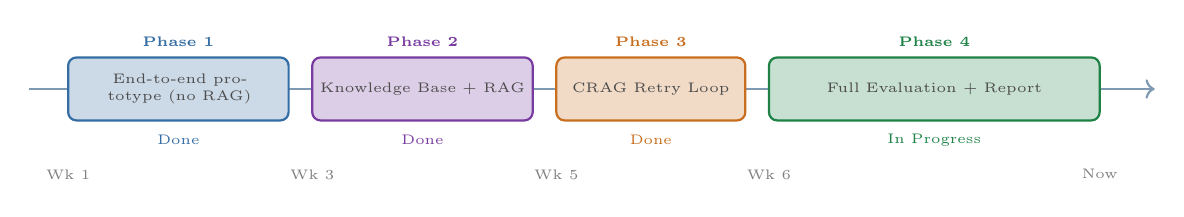
\begin{tikzpicture}[font=\scriptsize]
    % Horizontal axis
    \draw[->,thick,sfaxblue!50] (-0.3,0) -- (14,0);
    % Phases
    \foreach \x/\w/\col/\ph/\desc/\done in {
      0.2/2.8/moduleblue/Phase 1/End-to-end prototype (no RAG)/Done,
      3.3/2.8/modulepurple/Phase 2/Knowledge Base + RAG/Done,
      6.4/2.4/moduleorange/Phase 3/CRAG Retry Loop/Done,
      9.1/4.2/accentgreen/Phase 4/Full Evaluation + Report/In Progress
    }{
      \fill[\col!25, rounded corners=3pt] (\x,-0.4) rectangle (\x+\w,0.4);
      \draw[\col, thick, rounded corners=3pt] (\x,-0.4) rectangle (\x+\w,0.4);
      \node[font=\tiny\bfseries, color=\col] at (\x+\w/2, 0.6) {\ph};
      \node[font=\tiny, color=black!70, align=center, text width=\w cm]
        at (\x+\w/2, 0) {\desc};
      \node[font=\tiny, color=\col] at (\x+\w/2, -0.65) {\done};
    }
    % Week labels
    \foreach \x/\lbl in {0.2/Wk 1,3.3/Wk 3,6.4/Wk 5,9.1/Wk 6,13.3/Now}
      \node[below, font=\tiny, color=gray] at (\x, -0.9) {\lbl};
  \end{tikzpicture}
  \end{center}
  \vspace{0.3em}
  \begin{columns}[T]
    \begin{column}{0.5\textwidth}
\begin{lstlisting}[caption=Running the evaluation]
# Install
pip install -r requirements.txt

# Baseline (no API key needed)
python scripts/evaluate.py \
  --mode baseline

# Full evaluation
export ANTHROPIC_API_KEY="sk-..."
python scripts/evaluate.py \
  --mode full \
  --model claude-sonnet-4-6
\end{lstlisting}
    \end{column}
    \begin{column}{0.46\textwidth}
      \begin{block}{\faTools\ Technology Stack}
        {\scriptsize
        Python 3.13 $\cdot$ pytest (58 tests)\\
        ChromaDB $\cdot$ sentence-transformers\\
        Checkov $\cdot$ unified diff\\
        Anthropic SDK $\cdot$ OpenAI SDK\\
        OpenRouter (free Llama/Mistral)
        }
      \end{block}
    \end{column}
  \end{columns}
\end{frame}

% ================================================================
\section{Conclusion \& Perspectives}
% ================================================================

{
\setbeamertemplate{footline}{}
\begin{frame}[plain]
\begin{tikzpicture}[remember picture, overlay]
  \fill[sfaxdark] (current page.south west) rectangle (current page.north east);
  \fill[sfaxgold] ([yshift=-0.45\paperheight]current page.north west)
    rectangle ([yshift=-0.55\paperheight]current page.north east);
  \node[text=white, font=\Huge\bfseries] at (current page.center)
    {8. Conclusion \& Perspectives};
\end{tikzpicture}
\end{frame}
}

\begin{frame}{Contributions \& Future Work}
  \begin{columns}[T]
    \begin{column}{0.50\textwidth}
      \begin{exampleblock}{\faStar\ Contributions (In Progress)}
        \begin{enumerate}
          \item \textbf{Proposed agentic framework} aiming to close the\\
            detect $\to$ retrieve $\to$ generate $\to$ validate loop for IaC security
          \item \textbf{CRAG-based strategy} for IaC: query refinement guided by validator feedback (under evaluation)
          \item \textbf{4-layer evaluation plan} with 18 metrics (detection, retrieval, remediation, agentic)
          \item \textbf{Curated dataset}: 8 files, 27 smells, 62-category taxonomy
        \end{enumerate}
      \end{exampleblock}
    \end{column}
    \begin{column}{0.46\textwidth}
      \begin{block}{\faRocket\ Design Goals}
        \begin{itemize}
          \item External validator as the \textbf{judge} (planned)
          \item 4 IaC tools in one framework
          \item Adaptive RAG on retry
          \item 4 LLM backends, no lock-in (prototype tested)
        \end{itemize}
      \end{block}
      \vspace{0.4em}
      \begin{alertblock}{\faArrowCircleRight\ Remaining Work \& Perspectives}
        \begin{itemize}
          \item Complete LLM integration (Configs B, C, D)
          \item Explore GLITCH for Ansible/Chef
          \item Consider fine-tuning on GenSIAC
          \item Expand with real GitHub IaC repos
          \item Multi-agent architecture (long-term)
        \end{itemize}
      \end{alertblock}
    \end{column}
  \end{columns}
\end{frame}

% ----------------------------------------------------------------
% FINAL SLIDE
% ----------------------------------------------------------------
{
\setbeamertemplate{footline}{}
\begin{frame}[plain]

\begin{tikzpicture}[remember picture, overlay]
  \fill[titlebg] (current page.south west) rectangle (current page.north east);
  \fill[sfaxgold] ([yshift=-0.12\paperheight]current page.north west)
    rectangle ([yshift=-0.15\paperheight]current page.north east);
  \fill[sfaxgold] ([yshift=0.06\paperheight]current page.south west)
    rectangle ([yshift=0.09\paperheight]current page.south east);
  % Decorative circles
  \fill[sfaxblue!50, opacity=0.35]
    ([xshift=0.82\paperwidth, yshift=-0.5\paperheight]current page.west)
    circle (2.5cm);
  \fill[sfaxgold!40, opacity=0.25]
    ([xshift=0.88\paperwidth, yshift=-0.25\paperheight]current page.west)
    circle (1.2cm);
\end{tikzpicture}

\begin{columns}[T]
  \begin{column}{0.65\textwidth}
    \vspace{2em}
    \begin{center}
      {\color{sfaxgold}\Huge\textbf{Thank You}}\\[0.5em]
      {\color{white!60}\rule{7cm}{0.6pt}}\\[1em]
      % Author info box
      
\begin{tikzpicture}
        \node[fill=sfaxblue!40, draw=sfaxgold!60, rounded corners=5pt,
              minimum width=7cm, align=center, inner sep=10pt] at (0,0) {
          \begin{tabular}{@{}c@{}}
            {\color{sfaxgold}\Large\faUserGraduate}\\[4pt]
            {\color{white}\large\textbf{Ahmedou Yahye Kheyri}}\\[4pt]
            {\color{white!80}\small Master MRSI --- PFE 2025--2026}\\[2pt]
            {\color{white!70}\small \faChalkboardTeacher\
              Supervised by: \textbf{Prof.\ Hala Bezine}}\\[2pt]
            {\color{white!70}\small \faUniversity\
              Faculty of Sciences of Sfax}\\[2pt]
            {\color{white!70}\small \faCalendar\ April 2026}\\
          \end{tabular}
        };
      \end{tikzpicture}
    \end{center}
  \end{column}
  \begin{column}{0.32\textwidth}
    \vspace{3em}
    \begin{center}
      {\color{sfaxgold}\Large\textbf{Questions?}}\\[1em]
      \begin{tikzpicture}[font=\tiny]
        \foreach \i/\col/\ico/\lbl in {
          4/moduleblue/\faCode/3 modules done,
          3/accentgreen/\faCheckCircle/58 tests pass,
          2/modulepurple/\faDatabase/62-cat taxonomy,
          1/sfaxgold/\faFlask/27 labelled smells,
          0/moduleorange/\faServer/4 IaC tools
        }{
          \node[draw=\col!60, fill=\col!10, rounded corners=2pt,
                minimum width=2.8cm, minimum height=0.45cm,
                align=center, font=\tiny] at (0, \i*0.55)
            {{\color{\col}\ico}\ \lbl};
        }
      \end{tikzpicture}
    \end{center}
  \end{column}
\end{columns}
\end{frame}
}

\end{document}
